\chapter{Sistema propuesto (teoría y simulaciones)}

Se propone un sistema de comunicaciones óptico con una estructura de hub como se aprecia en la figura \ref{fig_hub}. Utilizando este Diseño físico con una etapa adicional de codificación y correccion de errores. El hub central es una etapa totalmente óptica que puede o no estar amplificada. Con la amplificacion optica se incrementa notablemente el rango, de 5 km a mas de 20 km.
La pila de codificación se detalla en la figura \ref{fig_stack} donde puede verse un arreglo convencional, excepto en la ultima 

\begin{figure}[t]
\centering
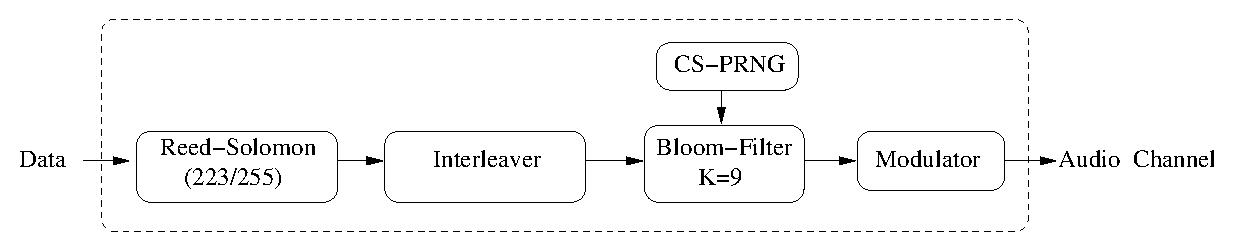
\includegraphics[width=0.9 \textwidth]{Soft-stack2.eps} 
\caption{Etapas del sistema de comunicaciones}
\label{fig_comstack}
\end{figure}

\section{Códigos correctores de errores}

Todo sistema de comunicaciones posee errores que deben ser corregidos antes que los datos sean procesados. Una técnica muy utilizada es la de utilizar un algoritmo de detección y retransmisión.
La idea de un código corrector de errores esta relacionada con la técnica de espectro expandido, siendo ambas métodos que ayudan a la transmisión de la información reduciendo la entropía de la información transmitida, o lo que es lo mismo, aumentando la redundancia de la información. En particular, los sistemas de comunicaciones modernos hacen uso de los métodos de Forward Error Correction (FEC) que no necesitan de retransmisiones.



\subsection{Reed-Solomon}
Se utilizo un codigo de Reed-Solomon standard 223/255, esto significa que se tienen 32 bytes de paridad por cada 223 bytes de datos, y se pueden corregir hasta 16 bytes. Se utilizo la librería de Phil Karn, y no se utilizaron los bits de sindrome para mejorar la correccion. Todo error conocido es descartado.
Con posibilidad de error de simbolo P, la posibilidad de error de un codigo reed-solomon R(n/k) es:
$$P_{rs}= \sum_{k=(\frac{n-k}{2}+1)}^{n} \binom{L}{i} * P^{i} * (1-P)^{L-i} $$

\subsection{LDPC}
El esquema de corrección de errores LDPC (Low Density Parity Check) es muy utilizado actualmente debido a su gran capacidad de corrección de errores, en algunos casos muy cercana a la máxima capacidad teórica del canal.
Antes de ahondar en la descripción de este algoritmo cabe aclarar que a pesar de ser utilizado para ciertos modelos durante la primera fase de la investigación, fue descartado en la versión final por un modelo mas simple y con menos requerimientos de hardware que presenta una performance similar desde el punto de vista de corrección de errores.
Básicamente es un código lineal que utiliza una matriz de paridad grande y dispersa.
La matriz H es tal que cualquier codeword valido x cumple con $H*x=0$

\paragraph{LDPC: Generador de matriz}
La matriz generadora puede crearse facilmente si H es de la forma $[D|I]$, simplemente formando la matriz:
$$G=[I|D']$$
Donde D' es la transpuesta de la matriz D
Para la generacion de la matriz se opto por utilizar un algoritmo random y luego aplicando algunos tests, para lograr una matriz sistemática de rate entero (1/2, 1/3, etc.)
Para verificar se G genera vectores cuya matriz de paridad es H, puede verificarse que:
$$ H*G'=0 $$

Podemos definir la matriz de paridad H como una matriz de paridad que tenga mas de 3 unos por fila y una cantidad similar por columna. Buenos resultados se obtienen a partir de matrices de 200x100.
Se puede comenzar por una matriz vacía $H = 0$ del tamaño deseado, y ir agregándole unos al azar. Cierto análisis es necesario para garantizar que no se cumplan ciclos y que la cantidad de unos por columna y por fila es la deseada. De esto se encargan los algoritmos llamados evencol y evenrow.

El generador puede generar matrices de cualquier tamaño, de esta manera:

$$ ./genMatrix <width> <height> <ones per row>$$

La matriz se genera en la salida estandard. El formato es el utilizado por la libreria boost:ublas.

NOTA: La matriz siempre esta compuesta de simbolos en GF(2) (O sea, ceros y unos)

\paragraph{LDPC: encoder}

El vector inicial se toma de la entrada estandard y el codeword se emite en la salida estandard. La sintaxis es muy sencilla:

$$ ./ldpcen <matriz> < in >out $$
\paragraph{LDPC: decoder}
Si se invoca este filtro mediante el nombre decodificador, tomara el codeword de la entrada estandard, aplicara el algoritmo de belief-propagation (Hard-decision) y se emite el vector original por la salida estandard:
La diferencia radica que en nuestro caso, al ser un canal asimetrico no se permite el bit-flip de un valor cero a un valor uno, ya que es imposible que se produzca ese error.
La linea de comando es la siguiente:

$$ ./ldpcdec <matriz> <in >out $$

La conversion codeword->vector es sencilla, ya que al ser un codigo sistemático solo se necesita eliminar la parte del vector que representa la paridad añadida.

Se generaron muchas matrices, desde 256x128 hasta matrices muy grandes de 10000x5000, pero el tiempo de decodificacion crece enormemente para matrices grandes.

\paragraph{LDPC: optimizacion}

Debido a la naturaleza iterativa del decodificador ldpc, pronto se convirtio en el cuello de botella de la simulacion. Para acelerar el sistema, se opto por realizar la siguiente optimizacion:
LDPC consta basicamente de varios loops, dentro de los cuales se accede a la matriz de paridad, y a otras matrices que acumulan datos intermedios. Primeramente la implementacion fue realizada como mencionamos utilizando boost:ublas, pero luego se comprobo que una implementacion utilizando arrays de C era hasta 3 veces mas rapida.
Luego se procedio a realizar un algoritmo de ``unrolling'' de estos loops, generando codigo especifico a una matriz dada, sin ningun tipo de loop. Obviamente este codigo es mucho mas grande, pero la aceleracion provista es aun mayor, del orden de 8 veces mas rapido que en implementaciones iniciales.
La manera de invocar el generador de codigo es la siguiente:

$$ ./genLdpcDecoder matriz  > decodeGen.h $$

El archivo generado decodeGen.h es el decodificador especifico para la matriz dada. Este header de C es luego incluido desde el decodificador ldpcenc.cpp y compilado. Al ser generalmente un archivo de un megabyte para una matriz pequeña de 1024x512, el proceso de compilacion el largo y requiere de mucha memoria.
Por otra parte, no se optimizo el proceso de codificacion ldpc, ya que consiste solo de una multiplicacion de un vector por una matriz, y es una de las tareas en la que boost:ublas es especialmente eficiente.

\section{Canal Z con filtros de bloom}
En esta sección vamos a modelar el canal por el cual estamos transmitiendo datos, específicamente el modelo de ruido del mismo. Es este modelo de ruido, distinto de canales convencionales como por ejemplo ruido Gaussiano, que nos permite innovar en el diseño de algoritmos.
Empezaremos primeramente estudiando un modelo simplificado del canal por el cual vamos a trasmitir, un simple canal simétrico binario, para despues ahondar en un caso especial de este mismo, denominado Canal Z.
\begin{figure}[t]
  \begin{center}
    \includegraphics[scale=0.43]{capacidad/canalBinario.png}
  \end{center}
\caption {Canal binario: esquema de probabilidad}
\label{fig:canbin}
\end{figure}

Para calcular el ruido en un canal simétrico binario, calculamos la probabilidad de no-colision que tendra un usuario determinado, ya que las colisiones seran el ruido del canal (En esta etapa no consideramos otros tipos de ruido que pueda tener el canal físico).

\noindent Cantidad de slots por trama: $m$
\noindent Cantidad de usuarios: $n$

\noindent Probabilidad de no colisión para un usuario en un canal simétrico:
\begin{equation}
P_{nc}=\left(\frac{m-1}{m}\right)^{n-1}
\end{equation}


\noindent Probabilidad de no colisión para un usuario en un canal óptico:
\begin{eqnarray}
P_{nc} & = & P(1) \cdot P_{nc}(1) + P(0) \cdot P_{nc}(0) \\
P_{nc} & = & \frac{1}{2} \cdot 1 +  \frac{1}{2} \cdot \sum_{i=0}^{n-1} 
C^{n-1}_{i} \left(\frac{m-1}{m}\right)^i  \left(\frac{1}{m}\right)^{n-1-i}  \left(\frac{1}{2}\right)^{n-1-i} 
\end{eqnarray}

\noindent Donde $\left(\frac{m-1}{m}\right)^i$ es la probabilidad de no
colisión de $i$ canales (se suma para todo posible número de canales no
colisionando: $1\leq i\leq n$, que están en otro slot), $
\left(\frac{1}{m}\right)^{n-1-i}$ es la probilidad de colisión de los restantes
$n-1-i$ (estos están en el mismo slot que el canal actual, el `$-1$' es para no
contar el canal actual), y la colisión se produce cuando los otros canales
transmiten $1$ cuya probabilidad es $\left(\frac{1}{2}\right)^{n-1-i}$. El
factor $C^{n-1}_{i}$ suma sobre todas las combinaciones posibles de canales no
colisionando, que son hechos independientes.

\noindent Teniendo en cuenta que $ \sum_{i=0}^{n-1}
C^{n-1}_{i} \left(\frac{m-1}{m}\right)^i  \left(\frac{1}{2m}\right)^{n-1-i}$ es la potencia $n-1$ de un binomio, reemplanzando tenemos
\begin{eqnarray}
P_{nc} & = & \frac{1}{2} +  \frac{1}{2} \cdot \left(\frac{m-1}{m} + \frac{1}{2m} \right)^{n-1} \\
P_{nc} & = & \frac{1}{2} +  \frac{1}{2} \cdot \left(1- \frac{1}{2m} \right)^{n-1} \\
P_{nc} & \simeq & \frac{1}{2} +  \frac{1}{2} \cdot e^{-1/2} 
\end{eqnarray}

\noindent Donde la última aproximación vale para $n=m$ y $n$ grande.


\vspace{5mm}

\noindent Para el caso de {\em bloom} filters con $k$ filtros\footnote{Se envían $k$ repeticiones del bit en canales distintos, entonces basta que sólo uno de ellos sea 0 para que recibamos un 0 en un canal óptico.} la probabilidad de no colisión es:
\begin{eqnarray} 
P_{nc}^{k} & = &  P(1) \cdot P_{nc}^{k}(1) + P(0) \cdot P_{nc}^{k}(0)\\ \label{Pnc_k}
\end{eqnarray}
Sabiendo que la probabilidad de no colisión para el 0 es:
\begin{eqnarray}
P_{nc}^{k}(0) & = & 1 - \big(P_{c^k}(0)\big)^k 
\end{eqnarray}
Pero la probabilidad de colisión para el 0 cuando se transmiten $k$ copias es:
\begin{eqnarray}
P_{c^k}(0) & = & 1 - \big(P_{nc^k}(0)\big)  \enspace,
\end{eqnarray}
y que además la probabilidad de no colisión para los $k$ slots del bloom
filter es
\begin{eqnarray}
P(\mbox{no col.} k) &=& P(\mbox{no col.}1)\cdot P(\mbox{no col.}2)\cdot P(\mbox{no col.}3)\cdots P(\mbox{no col.}k)\\
&=&\left(\frac{m-1}{m}\right)\cdot\left(\frac{m-2}{m-1}\right)\cdot\left(\frac{m-3}{m-2}\right)\cdots\left(\frac{m-k}{m-(k-1)}\right)\\
&=& \frac{m-k}{m} \enspace.
\end{eqnarray}
Luego la probabilidad de colisión con alguno de las $k$ copias del bit es
\begin{eqnarray}
P(\mbox{col.}k)&=& 1-P(\mbox{no col.} k)\\
&=& 1-\frac{m-k}{m}\\
&=& \frac{k}{m} \enspace.
\end{eqnarray}
Entonces reemplazamos y calculamos:
\begin{eqnarray}
P_{c^k}(0) & = & 1 - \left(\sum_{i=0}^{n-1} C^{n-1}_{i} \left(\frac{m-k}{m}\right)^i \left(\frac{k}{2m}\right)^{n-1-i} \right)  \\
& = &  1-\left( 1-\frac{k}{2m}\right)^{n-1}
\end{eqnarray}
Reemplazando esta ecuación en~\ref{Pnc_k} obtenemos:
\begin{eqnarray}
P_{nc}^k & = & \frac{1}{2} + \frac{1}{2} \left( 1- \left( 1- \left( 1- \frac{k}{2m} \right)^{n-1}  \right)^{k}  \right) 
\end{eqnarray}

Sin embargo, este calculo es incorrecto, comparandolo con los datos que da el simulador. La formula entrega valores de error menores con respecto a los reales, como se observa en la figura. 
Los trazos del mismo color corresponden a el mismo K con azul(K=1), verde (K=2) y rojo(K=4). M=256

\subsection{Entropía}

Comenzemos por lo básico:

Segun Shannon, el \textbf{contenido de informacion} h(x) de un suceso x dada la posibilidad que suceda P(x) es:
$$ h(x) = log_{2}\left(\frac{1}{P(x)}\right) $$

Y la entropia de un conjunto A, H(A) se define simplemente como el promedio del contenido de información:

$$ H(A) = \sum_{x E A_{x}} P(x)log_{2}\left(\frac{1}{P(x)}\right)$$

En un canal binario solo dos sucesos existen, uno con probabilidad p, y otro con probabilidad 1-p, por lo tanto para p siendo la probabilidad de error:

$$ H(p) = -p log_{2}(p)-(1-p)log_{2}(1-p) $$

\subsection{Entropia condicional}

Vamos a analizar la entropia de dos conjuntos X de entrada y Y de salida interrelacionados.

La entropia condicional de X dado $y=b_k$ donde $b_k$ es un valor dado, es la entropia de la distribucion de probabilidad $P(x|y=b_{k})$:
$$H(X|y=b_{k}) = \sum_{x \in A_{x}} P(x | y=b_{k})\log_2\left(\frac{1}{P(x | y=b_{k})}\right) $$

La entropia codicional de X dado Y es el promedio, sobre y, de la entropia condicional de X dado y:
$$H(X|Y) =  \sum_{xy \in A_{x}A_{y}} P(x,y)\log_2\left(\frac{1}{P(x,y)}\right) $$

\subsection{Información mútua}
La información mútua entre X e Y es:
$$I(X;Y) = H(X)-H(X|Y)$$
Mide el promedio de reduccion de la incertidumbre acerca de x que resulta de saber el valor de y, o viceversa: la cantidad promedio de informacion que x revela acerca de y.

\subsection{Capacidad de canal}

La capacidad C de un canal discreto sin memoria es :

\begin{equation}
C = \max_{{\cal{P}}_x} I(X;Y) 
\end{equation}

O sea, la máxima información mutua entre los alfabetos X de entrada e Y de salida.
Para hallar el maximo podemos derivar $I(X;Y)$ con respecto a la probabilidad $P_x$.
Para un canal binario asimétrico sin memoria con probabilidad de error $p$, la capacidad máxima $C$ es:

\begin{equation}\label{Cap}
C = 1 - H(p) 
\end{equation}

Si expandimos H(p) en \ref{Cap}:

$$ c = 1-\left(p \times \log_2\left(\frac{1}{p}\right) + (1-p) \cdot \log_2\left(\frac{1}{1-p}\right)\right) $$
Simplificada:
$$ c = 1 + p * \log_2(p) + (1 - p) * \log_2(1-p) $$

Sin embargo esta capacidad es menor que la que realmente tenemos en nuestro canal, ya que un Z-channel se adecua mayormente a los medios de transmisión ópticos. Describiremos en detalle este caso especial en la siguiente sección.

\subsection{Canal Z}
Un canal Z (Z-channel) difiere de un canal binario, ya que las probabilidades de bit-flip son asimetricas.
Los Z-channel se usan generalmente para modelar sistemas de transmision opticos.

\begin{figure}[th]
  \begin{center}
    \includegraphics[scale=0.5]{capacidad/zchannel}
  \end{center}
  \caption{Diagrama: Z-channel}
  \label{fig:Gal}
\end{figure}

Para un Z-channel, la distribucion de probabilidades de I(X;Y) es diferente, por lo que obtenemos un máximo diferente:

$$ C_{Z} = 1 - \left(\frac{1}{2}*H(p)\right) $$ \cite{tallini}

Por lo tanto,

$$ C_{Z} = \log_2\left(1+(1-p) p^{p/(1-p)}\right) $$


\begin{figure}[th]
  \begin{center}
    \includegraphics[scale=0.9]{capacidad/comparacionBZ}
  \end{center}
  \caption{Diagrama: Azul: Capacidad de canal binario Verde: Capacidad de canal Z}
  \label{fig:CompBZ}
\end{figure}


\subsection{Filtros de bloom}
As discussed in section 2, this leads to collisions. Since the modulation format is OOK, only transmitted ‘1’s can interfere with ‘0’s.
This behaviour can be modelled as a Z-channel because the superposition of individual light pulses representing ‘1’s
can only be identified as a ‘1’, but a received ‘0’ is an unmistakable sign of the absence of pulses in a given time slot.
We found that the Bloom filter [2] provides a convenient structure to correct for errors in this type of channel. This
technique is borrowed from hashing algorithms and is used to test whether an element is member of a given set. The
way that we implement this algorithm relies on copying every bit in K slots of the transmitted frame. On the receiving
end it is sufficient to receive a single ‘0’ out of K copies in order to correctly retrieve the original transmitted ‘0’,
whereas collisions have no effect on ‘1’s.

\section{Espectro ensanchado}

Repetido en \ref{espectroensanchado} ??
\subsection{Time-hopping con filtros de bloom}

\section{Minimización de peso de Hamming}
%% extraido de dline-pub.text

Repasando, el esquema propuesto basado en time-hopping CDMA se basa en la interferencia entre símbolos para obtener confidencialidad, ya que los datos de los otros usuarios actuan efectívamente como ruido.
La interferencia inter-símbolo, como fue discutida en la seccion \ref{principle}, causa errores que debe ser corregidos. Como dichos errores reducen el ancho de banda utilizable del canal, es deseable reducir la interferencia hasta un punto donde se maximize, sin comprometer la seguridad del sistema. Para reducir la interferencia, no es aconsejable modificar o introducir patrones en el generador criptograficamente seguro de numeros aleatorios, ya que comprometeria la seguridad de todo el sistema al introducir predictabilidad en las posiciones de los símbolos (Ej. usando códigos ortogonales como en Ref.~\cite{Nadarajah2006}.), efectivamente dejando de ser criptograficamente seguro.
En lugar de esto, se adopto una estrategia que aprovecha el echo que un sistema óptico puede ser modelado como un canal-Z.

%This channel presents a Shannon limit of $ C_{Z} = \log_2\left(1+(1-p) p^{p/(1-p)}\right),$ where $p$ is the probability of error~\cite{Tallini:02}.

Esta propuesta, y aqui esta el nucleo de la invencion propuesta en esta tesis, es la de aprovechar la naturaleza asimetrica del este tipo de canal, en donde solamente el símbolo ``1'' causa interferencia, ya que los ``0'' no se interfieren. \footnote{Aunque en un sistema óptico real, existe efectivamente una pequeña diferencia ya que un ``0'' nunca es representado con una potencia de laser de cero watts.}
En otras palabras, la interferencia de un canal-Z es proporcional al peso de hamming del símbolo transmitido.
El peso de Hamming de un símbolo es simplemente la cantidad de bits en ``1'' del mismo. El algoritmo de Minimización de peso de Hamming consiste en una codificación en donde cada símbolo binario es convertido en un equivalente de mayor longitud, tieniendo solamente una mínima cantidad de dígitos en ``1''. Aplicando esta codificación que minimiza el peso de Hamming y transmitiendo el símbolo resultante, se obtiene una menor interferencia en un canal Z.
Intuitivamente, expandir el símbolo original a uno de mayor longitud decrementaria el ancho de banda del canal; pero como las simulaciones numéricas muestran (ver sección \ref{simulations}) a medida que la interferencia inter-símbolo se reduce, el ancho de banda adicional utilizado por los algoritmos de FEC tambien se reducen, compensando por el incremento del largo del símbolo y logrando un mayor ancho de banda neto del sistema.
Podemos decir que un número binario normal de largo L posee un peso variable de Hamming, con L/2 siendo el promedio, cero siendo el mínimo y L siendo el máximo peso de Hamming.
La técnica de reduccion de peso de Hamming (HW) da buenos resultados reduciendo a HW=2, logrando un buen balance entre la reducción de interferencia y el largo de símbolo.
Adicionalmente, es deseable en un sistema de seguridad que no se revele ninguna información acerca de los símbolos transmitidos. Por ejemplo si transmitieramos el número cero, representado por todos sus dígitos en cero, seria trivial identificarlo sin importar si se aplica cualquier tipo de time-hopping. Para evitar estos ataques que utilizan estadísticas acerca del peso de hamming, la codificación exige que el peso de hamming sea fijo en todos los símbolos. Esto causa una ligera perdida en el ancho de banda pero hace imposible inferir cualquier tipo de información acerca del símbolo transmitido analizando estadisticas de tráfico de los datos transmitidos.

\begin{table}[t]
\begin{center}
\begin{tabular}{c c c}
Datos & entrada HW= 0 to 3 & Expandida HW=2\\
\hline\hline
0 & 000 & 00011\\
1 & 001 & 00110\\
2 & 010 & 00101\\
3 & 011 & 01100\\
4 & 100 & 01010\\
5 & 101 & 01001\\
6 & 110 & 10001\\
7 & 111 & 10010\\
\end{tabular}
\caption{Tambla de minimización de Hamming para símbolos de 3-bits}
\label{hwtable}
\end{center}
 \end{table}
 
\section{Expansión de símbolo}
La minimización del peso de hamming conlleva una necesaria conversión del símbolo original a otro que necesariamente tendra mayor longitud, o sea, una expansión del símbolo.
Esta operación puede realizarse de muchas maneras, pero un algoritmo muy eficiente es utilizar una tabla de lookup (ver tabla~\ref{hwtable}), donde un símbolo de largo L es utilizado como el índice en la tabla, y el resultado es el símbolo expandido, que tiene un largo N\textgreater L.
Por motivos prácticos y de optimización, es deseable que L sea 8 u 16 bits, por lo que la tabla contendrá 256 o 65536 entradas respectivamente.
Al aplicar la minimización de peso de hamming a símbolos de 8 o 16 bits de longitud, son necesarios 256 o 65536 símbolos de salida con un HW=2. En el caso de símbolos de entrada de 8 bits, la longitud del símbolo de salida sera de 363 bits, mientras que para 8 bits de entrada, el simbolo expandido con HW=2 tendra 24 bits de longitud.
Puede observarse que el número de símbolos únicos con HW=2 y N=363 no es exáctamente 65536 sino 65703, esto significa que existen muchas tablas de expansión.
La tabla seleccionada y el orden de la misma no son importantes para el resultado final, observando la condición que dos nodos comunicandose deberan utilizar idénticas tablas.
%In general more bits transmitted per frame the more efficient the protocol will be. \textbf{PORQUE IN GENERAL? CUANDO FALLA?} 


\section{Sistema completo}
%% De orte.tex
The proposed system is composed of an access layer, where CDMA and error correction are implemented, and a physical layer based on an optical network with certain similarities to PONs. 
The access layer is implemented using time-hopping CDMA, where each of the $128$ possible ONUs sends bits in a slot chosen randomly from a frame of $356$ slots; therefore
collisions between different ONUs will happen and error correction must be used to guarantee error-free data transmission. 
Notice that the synchronization is performed at the bit slot level only because transmission of each ONU is random, in contrast to TDMA where synchronization is also performed at frame level. 
Moreover, each ONU can send data at any time, in contrast to TDMA where
ONUs usually send data continuously; this feature resembles transport by Ethernet frames.
A certain ONU $X$ can receive messages from an ONU $Y$ if $X$ has the
{\em key} of $Y$, and vice versa. Therefore, if a certain group of ONUs
were to communicate over a VLAN, it is required that everyone in the group
knows each others' {\em keys}.
ONUs' data streams are encoded with the following error correction techniques (Fig. \ref{arch:chain}):
 Reed-Solomon ($223/255$) and LDPC ($1024\times512$ matrix) algorithms (see \cite{Moon:05} and references therein), and bloom-filters with $K=4$~\cite{Bloom70space/timetrade-offs}.
The choice of these correction algorithms was heavy influenced by
modeling the optical fiber as a Z-channel, having a Shannon limit of $ C_{Z} = \log_2\left(1+(1-p) p^{p/(1-p)}\right),$ where $p$ is the probability of error. 
This capacity limit is larger than that of a symmetric memoryless binary channel \cite{Tallini:02}.

\section{Aplicación en distintos medios físicos}
\subsection{Redes ópticas}
% de orte.text
\begin{figure}[!t]
  \centering
    \includegraphics[width=3in]{orte01.pdf}
    \caption{Proposed network design: Access Layer}
    \label{arch:chain}
\end{figure}
% Fiber		Es grave el efecto de la dispersion?  Sugerimos dispersion shifted G.653? O son muy caras?
% splitter	No 1x128 commercially available (attenuation $\leq 27\,dB$)
% DFB		http://cess-dk.com/gfx/upload/PX2-1541SF.pdf ( min $\simeq-1\,dB$)
% APD		http://pdf.dzsc.net.cn/200810212/286762.pdf ( max $\simeq-27\,dB$)
% EDFA		http://www.lambdaphoto.co.uk/pdfs/EDFADatasheet.pdf

The proposed physical layer topology is that of a star (see Fig.
\ref{arch:fig1}) where optical splitters redistribute traffic coming
from each ONU to all the rest allowing point-to-multipoint as well as
point-to-point communications between $128$ ONUs.
%Traffic redistribution is made by optical splitters at the redistribution hub that introduces high attenuation to optical streams.
An Erbium-Doped Fiber Amplifier (EDFA) located in between splitters at
the optical hub increases optical power to overcome network losses.  RZ
modulated optical signals generated at each ONU, of up to $10$~Gbps by a
$2$~dBm $1550$~nm DFB-laser, are transmitted up to $10$~km upstream by a
standard single-mode optical fiber (ITU-T G.652) to the optical hub.

In this hub a $128\times 1$ splitter merges traffic from all ONUs that is then redistributed by a $1\times 128$ splitter channeling back merged traffic to each ONU through a downstream fiber identical and parallel to the upstream fiber.
Splitters' attenuation ($\simeq25$~dB each) contribute, as well as fiber attenuation and insertion losses ($\simeq2$~dB and $\simeq1$~dB per stretch), to high total losses ($\simeq28$~dB at both upstream and downstream paths).
In order to provide signal amplification an EDFA ($\geq27$~dB gain) is placed between both splitters.
This EDFA increases merged traffic power at the first splitter output ($\simeq-26$~dBm `1' active Tx) delivering an adequate power level ($1$~dBm, `1' active Tx) at the second splitter input to provide ONU's receiver a power level for proper reception ($-27$~dBm, `1' active Tx) with a high sensitivity ($-28$~dBm) photodetector (PD).
The PD maximum optical power is not a concern as our simulations show that only up to ten `1' bits collide in any given single bit slot.
Even considering a constant EDFA gain, the PD input optical power would be lower ($-17$~dBm) than that commercial PDs withstand unharmed ($\sim -5$~dBm).
The bit `0' level at PD is given by the addition of the `0' bit transmitted 
by all $128$~ONUs.
The receiver decision threshold should be able to separate between this state and that of a single ONU transmitting a `1' bit.
As the bit `0' transmission power should be very low, imposing
restrictions on the DFB-laser extinction ratio.
The minimal required extinction ratio (`1'$/$`0' peak power ratio) is addressed in the numerical simulations explained next.
% As collisions occur in this scheme minimal powers are such for the case of a single active Tx in a bit slot. In a bit slot with collisions (two or more `1' bits) power increase could be a concern to APD operation
% Optical transmission is performed by a $2$~dBm $1550$ nm DFB-laser generating a
% $10$ Gb/s RZ modulated optical signal, that is transported by up to $10$
% km upstream fiber (ITU-T G.652) to a redistribution hub (see
% Fig.~\ref{arch:fig1}).
\begin{figure}[!t]
  \centering
    \includegraphics[width=3in]{orte02.pdf}
    \caption{Proposed optical network design: Optical Layer}
    \label{arch:fig1}
\end{figure}
% Upstream traffic from all ONUs are merged by a $128\times 1$ splitter and then again redistributed by another splitter $1\times 128$ that channels back merged traffic to each ONU through a downstream fiber identical and parallel to the upstream one.
% Splitters' attenuation ($\simeq25$~dB, estimated) contribute, as well as fiber attenuation and insertion losses ($\simeq2$~dB and $\simeq1$~dB per stretch), amount to high total attenuation ($\simeq28$~dB at each upstream and downstream paths).
% In order to make the system workable it is proposed to place a single EDFA optical amplifier ($\geq27$~dB gain) between both splitters.
% This EDFA rises merged traffic power at first splitter output ($\simeq-26$~dBm `1' active Tx) delivering enough power ($1$~dBm, `1' active Tx) at second splitter input to assure power reaching each ONU ($-27$~dBm, `1' active Tx) allows proper reception by a high sensitivity APD ($-28$~dBm).

\subsection{Redes acústicas}
% de newJIS_140512-1.pdf (paper JIS)
\begin{figure}[!t]
  \centering
    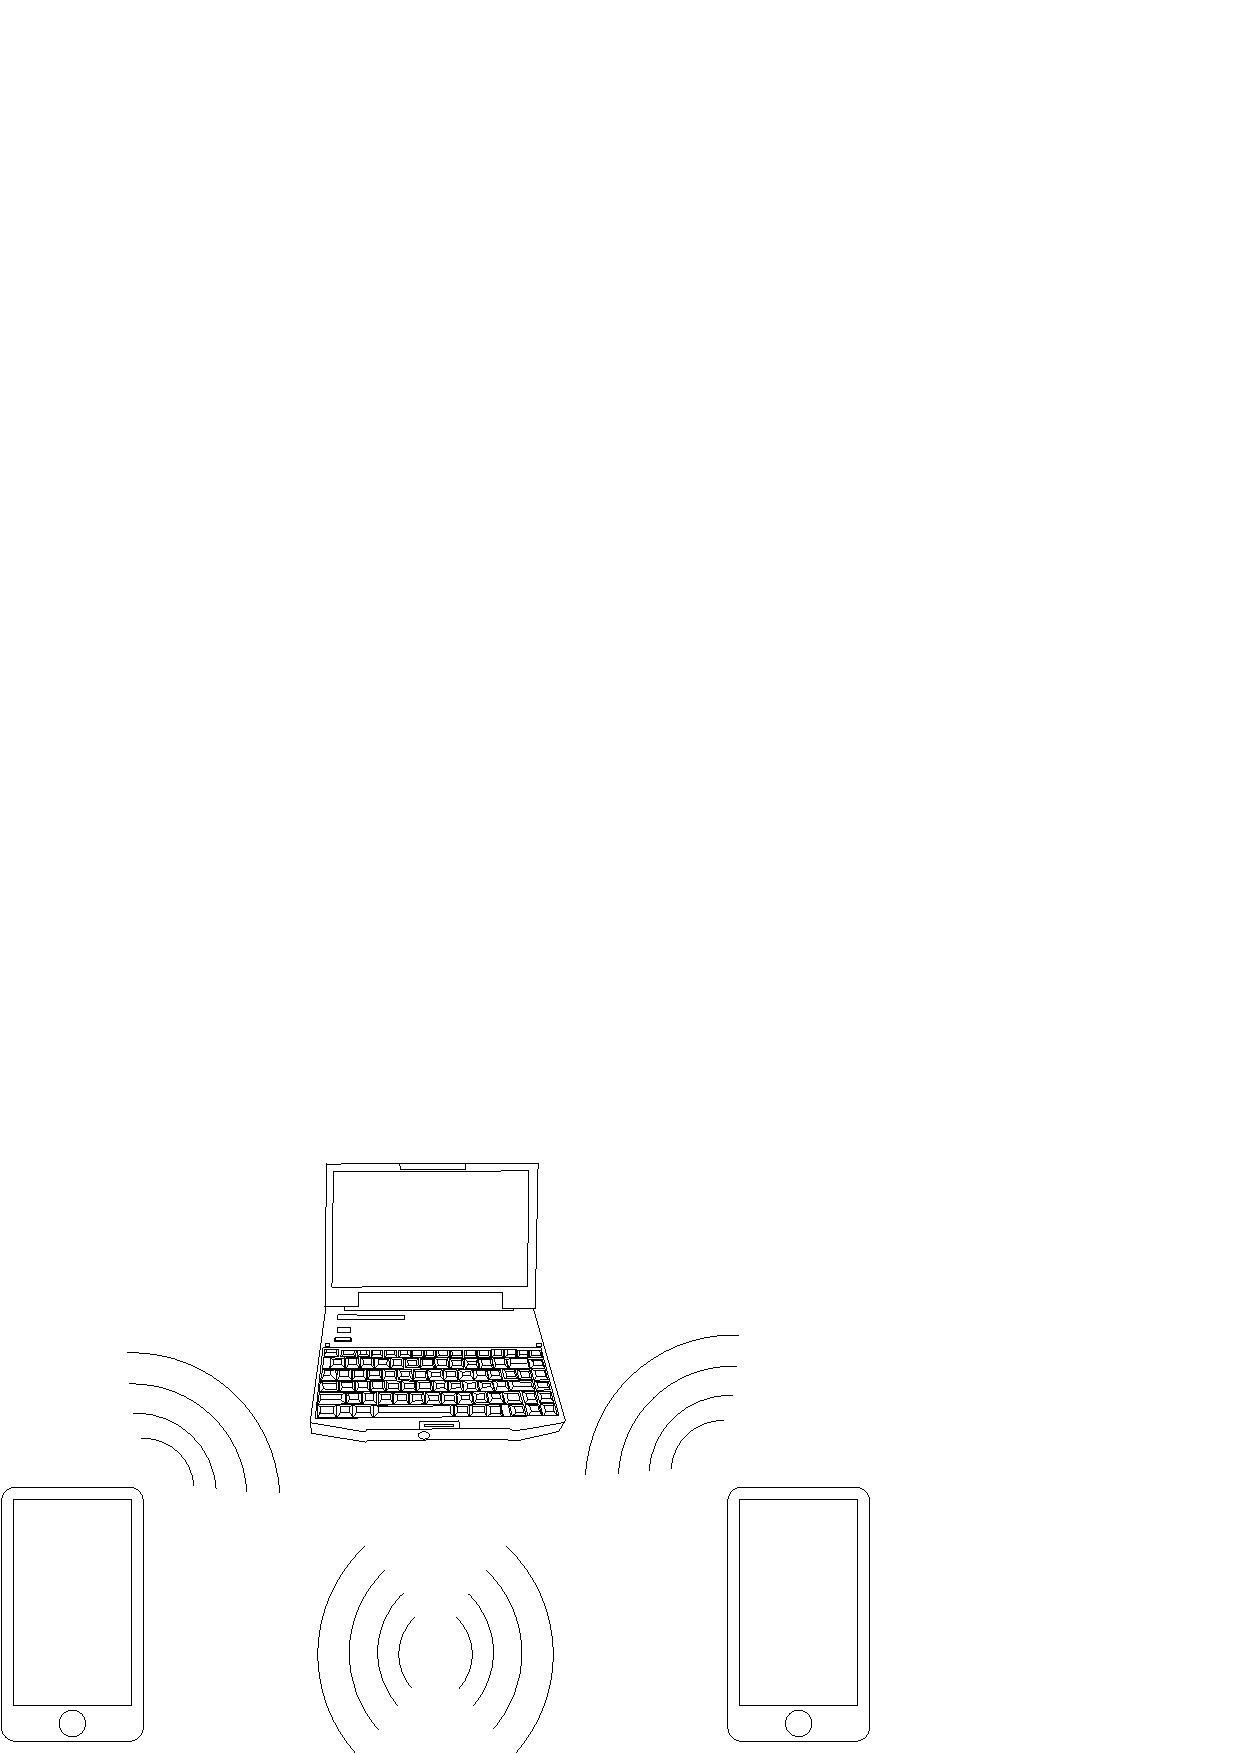
\includegraphics[width=3in]{compucelus.pdf}
    \caption{Proposed acoustic network may have heterogeneous nodes like cell-phones and personal computers.}
    \label{arch:chain}
\end{figure}


Optical links present as their main drawback the requirement of a clear line of sight between devices, a condition which cannot be guaranteed in some working environments. Moreover, they require the installation of additional light sensing hardware on devices not equipped with cameras, or even infra-red transceivers.
Acoustical communications, however, can operate using standard hardware microphones and speakers, ubiquitous on information devices [6]. Furthermore, line of sight is not required to establish links among nodes which can be placed up to a meter apart, emitting low volume audio.
Unlike other technologies, e.g., optical fiber communications, the broadcast nature of sound waves makes privacy safeguards an essential requirement. Several audio communication systems have been proposed [7], but to the best of our knowledge, the question of privacy has been addressed only in the application layer using security protocols. We present a physical layer approach to secure acoustical communications based on time-hopping CDMA, similar to those presented in references [8, 9]. In this work we present a point-to-point or point-to-multipoint secure acoustic network which has a short range and consumes a negligible amount of power, requiring no additional hardware on mobile clients.
Establishing a private link among previously un-paired mobile devices based on software privacy schemes requires some degree of user interaction that is usually neglected [5]. However, when privacy is dealt at the physical layer user intervention is minimized; that is the case in our proposal.
An envisioned application scenario for this technology is the validation of small financial transactions such as PoS (Point of Sale) or ATMs using an unmodified mobile device (e.g. a smartphone). A similar technology addressing these user cases is Near Field Communications (NFC) [10], a wireless protocol which requires specialized hardware not currently present in most mobile devices.

\subsection{Redes acusticas: Arquitectura}
The main advantage of the proposed system is the simplicity, just a sound emitter (speaker), a receiver (microphone) and a sound media channel are needed; and those are already available in computers, tablets and cell-phones. It is composed by Secure Time-hopping CDMA running over the sound media channel, error corrections algorithms, and a synchronization method. As a result, the system provides unidirectional users’ channels for point-to-point and multicast communications, while bi-directional communications can be established using two separate channels (i.e., two different CDMA codes in the same media), or by employing the same channel in half-duplex. The later proposition needs further developing work and falls beyond the scope of this paper.
We provide further details in the following subsections.

